\chapter{Upravljački program za temperaturni senzor ADT7301}

\section{Opis rada sklopa ADT7301}
	Sklop ADT7301 proizvođača Analog Devices je temperaturni senzor s integriranim 13-bitnim analogno-digitalnim pretvornikom i serijskim sučeljem SPI. Omogućuje mjerenje temperature u rasponu od -40\textcelsius{} do 150\textcelsius{}, s rezolucijom 0.03125\textcelsius{} i tipičnom preciznošću \textpm{} 0.5\textcelsius{} \citep{adt7301}. Blok dijagram sklopa prikazan je na slici \ref{fig:adt7301_blok_dijagram}.
	
	\begin{figure}[htb]
		\centering
		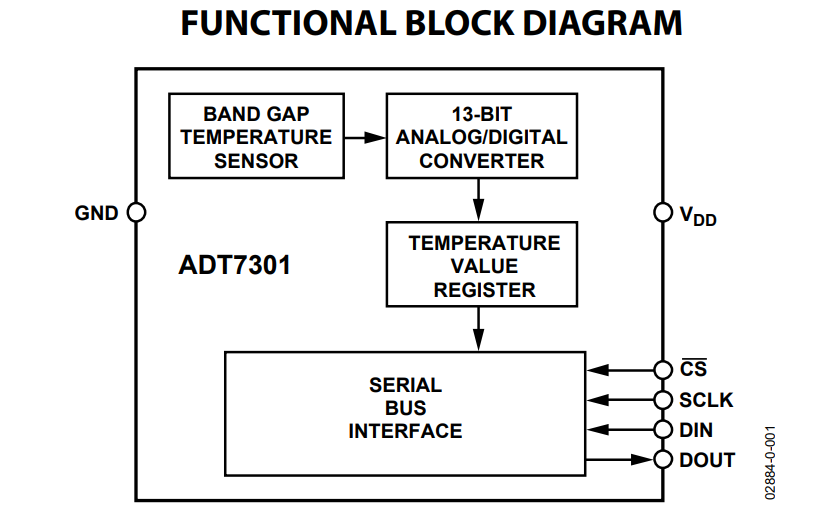
\includegraphics{slike/ADT7301_blok_dijagram.png}
		\caption{Blok dijagram sklopa ADT7301}
		\label{fig:adt7301_blok_dijagram}
	\end{figure}

	Senzor uzima mjerenja temperature svakih 1.5 sekundi, što je regulirano internim sklopom za mjerenje vremena \engl{timer}. Između dva mjerenja, napajanje analognog sklopovlja senzora je ugašeno te ono postaje neaktivno. Digitalno sklopovlje uvijek je aktivno, ali ako se pokuša pročitati vrijednost temperature više puta unutar jednog intervala mjerenja senzor će uvijek vraćati istu vrijednost (onu koju je izmjerio na početku intervala).
	
	Dodatna mogućnost sklopa je takozvani \textit{shutdown} način rada. U ovom načinu rada sklop troši vrlo malo struje (oko 1 \textmu{}A), što je korisno ako postoji dulje vremensko razdoblje u kojem se neće uzimati uzorci temperature. \textit{Shutdown} način rada omogućuje se upisom odgovarajućeg bita u kontrolni registar putem serijskog sučelja.
	
	Prilikom ispitivanja senzora u uvjetima sobne temperature, primijećeno je kako nakon nekoliko minuta kontinuiranog rada očitana temperatura počinje rasti, te može pokazivati vrijednosti čak i do 55\textcelsius{}. Zaključeno je da je navedeno posljedica zagrijavanja samog senzora. Zato je odlučeno da će se senzor između mjerenja stavljati u \textit{shutdown} način rada, kako bi se smanjila potrošnja struje, i samim time disipacija toplinske energije.

\section{SPI sučelje}
	Temperaturni senzor ADT7301 koristi SPI postavke CPOL = 1 i CPHA = 1, što znači da je takt visoke logičke razine u neaktivnom stanju i da se podatak čita na drugi brid takta (rastući).
	
	ADT7301 u stanju je istovremeno slati i primati podatke \engl{Full Duplex}. Na svojem priključku DOUT, koji je spojen na SPI liniju MOSI, sklop daje 16-bitni izlazni podatak na način da najznačajniji bit podatka izlazi prvi. Bitovi 15 i 14 su nule, bit 13 je bit predznaka, a ostali bitovi predstavljaju apsolutnu vrijednost očitane temperature. Na priključku DIN, koji je spojen na SPI liniju MISO, sklop prima 16-bitni podatak, gdje svi bitovi osim trećeg najznačajnijeg bita moraju biti nule. Treći najznačajniji bit je 1 u slučaju da se sklop želi staviti u \textit{shutdown} način rada nakon završetka ciklusa slanja, a 0 inače. Slika \ref{fig:adt7301_spi} prikazuje jedan SPI ciklus čitanja/pisanja.
	
	\begin{figure}[htb]
		\centering
		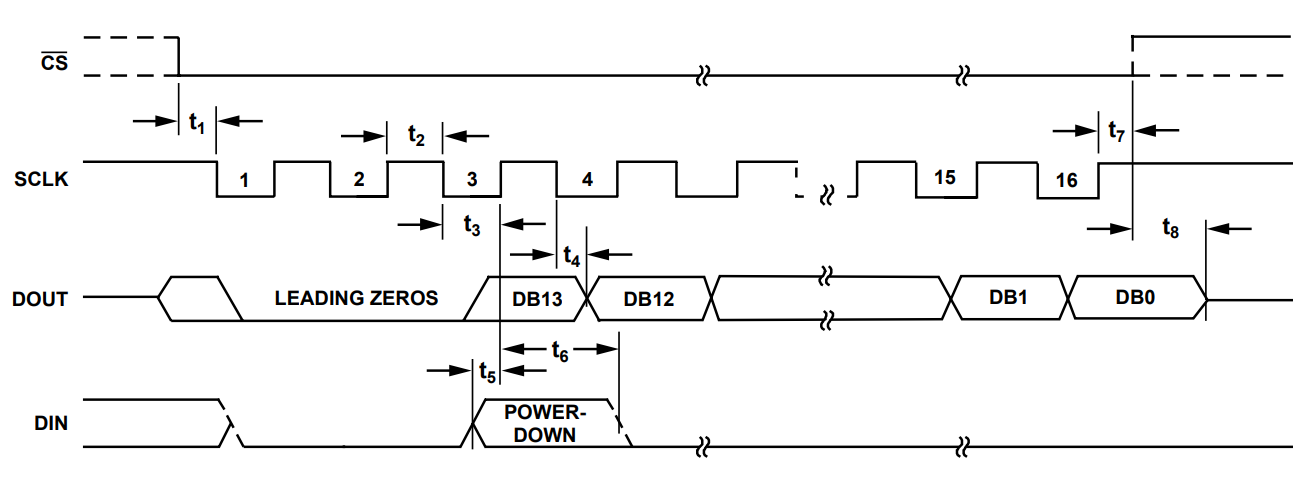
\includegraphics{slike/ADT7301_spi.png}
		\caption{Vremenski dijagram SPI komunikacije sklopa ADT7301}
		\label{fig:adt7301_spi}
	\end{figure}
	